\section{Introduction}
\label{sec:intro}

Automatic prompt optimization is most attractive where it is hardest: for small, locally deployed
models that cannot rely on a stronger model to critique their prompts \citep{zhang2024revisiting}.
\greater{} \citep{das2025greater} showed that such models can optimize their own prompts if the
signal is a true gradient of the task loss computed \emph{over the model's own reasoning}: the
model reasons under the current prompt, an extractor elicits its answer, and the gradient of the
answer loss with respect to one-hot prompt tokens shortlists token substitutions, which are then
verified by regenerating the reasoning.

Token coordinates are a poor match for how prompts are written and reviewed---as structured
documents with a task, a strategy, a procedure and an output contract, edited by rewriting,
deleting or inserting whole instructions. Lifting \greater{}'s signal to such edits poses a
technical problem, since edits of different lengths have no one-hot relaxation, and a conceptual
one: a structural edit changes the very reasoning the gradient is computed over. We solve the
technical problem exactly and then show that the conceptual one is decisive---and that it has a
principled fix.

\textbf{Contributions.}
\begin{itemize}
\item \emph{An exact calculus for structural edits} (\S\ref{sec:calculus}). All candidate rewrites
of all blocks share one sequence in parallel slots behind attention gates, with continuous slot
offsets realized as rotary rotations; every vertex---replacement, deletion, insertion and their
combinations---is exactly a real edited prompt, and one forward/backward pass estimates the effect
of every edit.
\item \emph{A preregistered diagnosis} (\S\ref{sec:diagnosis}). Across three models and eleven
proposal pools, \greater{}'s fixed-reasoning objective ranks LLM-proposed block edits in the wrong
direction ($8$ of $11$ pools; as a one-pass shortlist worse than random in $8$ of $11$), while
fresh evaluation is positive in $9$--$10$ of $11$. Under a deterministic reader, edits rewrite the
reasoning they are scored on, and verifying candidates on small minibatches picks noise.
\item \emph{A decomposition and a fix} (\S\ref{sec:theory}). An edit's effect on accuracy splits
exactly into a reasoning-distribution term and an answer read-off term; the fixed-reasoning
objective sees only the read-off term, which on the models' own samples is three to twenty times
smaller and, on wrongly answered questions, rewards reading against one's own reasoning. Exact
likelihood ratios of the model's own sampled reasoning recover the missing term without
generating under any candidate: \todo{H-dist / H-inc pooled results}.
\item \emph{End-to-end and at scale} (\S\ref{sec:experiments}). \todo{Stage C v2: dist vs
\greater{}-lifted vs random vs textual gradients at matched verification; official \greater{} with
gradient vs random shortlist; breadth over 21 BBH tasks, GSM8K and FOLIO.}
\end{itemize}

\begin{figure*}[t]
\centering
\resizebox{\textwidth}{!}{% Method overview: token-level relaxation (GReaTer) vs superposed typed blocks (GRAFT).
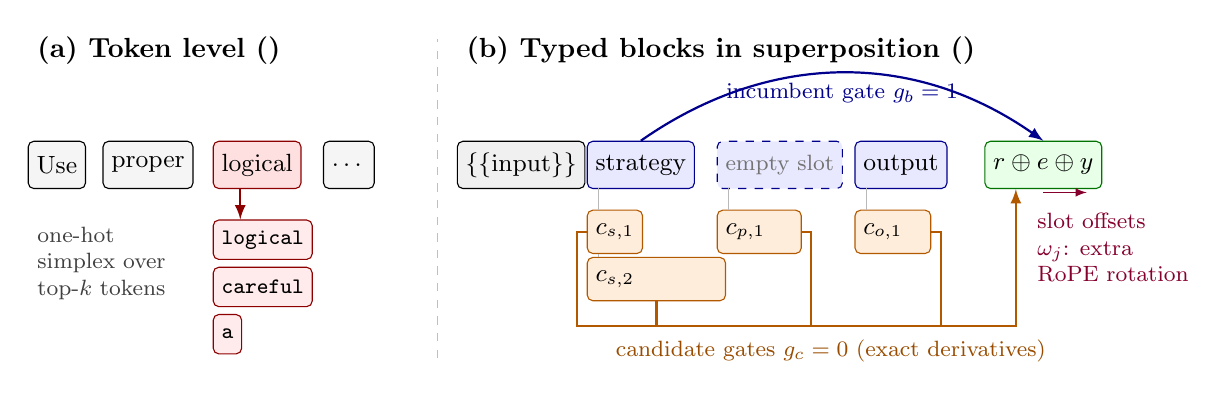
\begin{tikzpicture}[
  x=1cm, y=1cm, font=\small,
  box/.style={draw, rounded corners=2pt, minimum height=6mm, inner sep=3pt, anchor=west},
  tok/.style={box, fill=gray!8},
  alt/.style={box, fill=red!8, draw=red!55!black, minimum height=5mm, font=\footnotesize\ttfamily},
  frz/.style={box, fill=gray!12},
  inc/.style={box, fill=blue!9, draw=blue!55!black},
  cand/.style={box, fill=orange!14, draw=orange!70!black, minimum height=5.5mm},
  tail/.style={box, fill=green!9, draw=green!45!black},
  note/.style={font=\footnotesize, text=black!75, anchor=west, align=left},
  arr/.style={->, >=latex, thick},
]
% ---------------- (a) GReaTer ----------------
\node[anchor=west, font=\bfseries] at (0, 5.05) {(a) Token level (\greater{})};
\node[tok] (u) at (0, 3.6) {Use};
\node[tok] (pr) at (0.95, 3.6) {proper};
\node[tok, fill=red!12, draw=red!55!black] (lo) at (2.35, 3.6) {logical};
\node[tok] (re) at (3.75, 3.6) {\dots};
\node[alt] (a1) at (2.35, 2.65) {logical};
\node[alt] (a2) at (2.35, 2.05) {careful};
\node[alt] (a3) at (2.35, 1.45) {a};
\draw[arr, red!55!black] ([xshift=3.5mm]lo.south west) -- ([xshift=3.5mm]a1.north west);
\node[note] at (0, 2.35) {one-hot\\simplex over\\top-$k$ tokens};

\draw[gray!50, dashed] (5.2, 1.15) -- (5.2, 5.2);

% ---------------- (b) GRAFT ----------------
\node[anchor=west, font=\bfseries] at (5.45, 5.05) {(b) Typed blocks in superposition (\graft{})};
\node[frz] (x) at (5.45, 3.6) {\{\{input\}\}};
\node[inc] (s) at (7.1, 3.6) {strategy};
\node[inc, dashed, text=black!55] (p) at (8.75, 3.6) {\footnotesize empty slot};
\node[inc] (o) at (10.5, 3.6) {output};
\node[tail] (t) at (12.15, 3.6) {$r \oplus e \oplus y$};
% candidate lanes: each starts at its incumbent's first position
\node[cand] (c1) at (7.1, 2.75) {$c_{s,1}$};
\node[cand] (c2) at (7.1, 2.15) {$c_{s,2}$\,\rule{10mm}{0pt}};
\node[cand] (c3) at (8.75, 2.75) {$c_{p,1}$\,\rule{3mm}{0pt}};
\node[cand] (c4) at (10.5, 2.75) {$c_{o,1}$\,\rule{2mm}{0pt}};
\foreach \c in {c1, c3, c4} {\draw[gray!55] ([xshift=1.5mm]\c.north west) -- ++(0, 0.27);}
\draw[gray!55] ([xshift=1.5mm]c2.north west) -- ([xshift=1.5mm]c1.south west);
% incumbent gate
\draw[arr, blue!55!black] (s.north) to[out=35, in=145] node[pos=0.5, below, font=\footnotesize] {incumbent gate $g_b=1$} (t.north);
% candidate gates share a bus into the downstream tokens
\draw[orange!70!black, thick] (c1.west) -- ++(-0.12,0) |- (12.0, 1.55);
\foreach \c in {c3, c4} {\draw[orange!70!black, thick] (\c.east) -- ++(0.12,0) |- (12.0, 1.55);}
\draw[orange!70!black, thick] (c2.south) |- (12.0, 1.55);
\draw[arr, orange!70!black] (12.0, 1.55) -| ([xshift=4mm]t.south west);
\node[font=\footnotesize, text=orange!60!black, anchor=north] at (10.2, 1.5) {candidate gates $g_c=0$ (exact derivatives)};
\node[note, text=purple!70!black] at (12.7, 2.55) {slot offsets\\$\omega_j$: extra\\RoPE rotation};
\draw[->, >=latex, purple!70!black] (12.9, 3.25) -- (13.45, 3.25);
% The vertex and one-pass notes formerly drawn here are stated in the caption and in Section 3.
\end{tikzpicture}
}
\caption{\textbf{From token coordinates to typed blocks.} (a) \greater{} relaxes one prompt token
into the vocabulary simplex; its vertices are real tokens but every edit keeps the prompt's length
and structure. (b) Candidate rewrites of every typed block sit in parallel slots behind attention
gates, with continuous slot offsets realized as rotary rotations; every vertex is exactly a real
edited prompt.}
\label{fig:overview}
\end{figure*}
